% the first part of the document before the begin is called preamble
\documentclass[12pt, a4paper]{article}
\usepackage{graphicx}
\usepackage{hyperref}
\graphicspath{ {./images/} }
%
\author{Leonardo Valente}
\title{Sistemi Distribuiti}

\begin{document}
    \maketitle
    \tableofcontents
    \section{Introduzione}
    \subsection{Che cosa è un sistema distribuito?}
    
    Ci possono essere diverse definizioni di ''Sistema Distributo''.
    \begin{itemize}
        \item Definiamo un sistema distribuito come un insieme di componenti 
        Hardware e Software localizzati in una rete di computer che
        comunicano e coordinano le loro azioni solo passandosi messaggi.
        
        \item Un ''Sistema Distribuito'' è un insieme di elementi di computazione
        autonomi che appaiono all'utente come un singolo sistema coerente.
    \end{itemize}

    \subsection{Caratteristiche}
    Gli "elementi di computazione autonoma" di un SD, anche chiamati "Nodi"
    sono i device hardware oppure i processi software. Il fatto un SD debba sembrare
    un singolo sistema all'utente implica il fatto che tra i nodi ci deve essere un sistema
    di collaborazione.
    \\
    Quindi ogni nodo in quanto autonomo avrà la sua singola nozione di tempo. 
    Non esiste un clock globable per tutti i nodi.
    \\
    Questo porta quindi a problemi di sincronizzazione e di coordinamento.
    \\\\
    La parola chiave resta sempre: \textbf{Trasparenza}
    \\\\E' inevitabile il fatto che in qualsiasi momento solo parte del sistema fallirà.
    Nascondere questi fallimenti e il loro recupero è molto spesso difficile e in generale impossibile da nascondere.
    \\\\
    \textbf{Gestione della memoria?}
    
    \begin{itemize}
        \item Non c'è memoria condivisa.
        \item Comunicazione via scambio di messaggi.
        \item Ogni componente conosce solo il proprio stato e può sondare lo stato degli altri
    \end{itemize}
    \textbf{Gestione dell' esecuzione?}
    \begin{itemize}
        \item Ogni componente è autonomo.
        \item Il coordinamento delle attività è importante per il funzionamento di un sistema
        formato da più componenti.
    \end{itemize}
    \textbf{Gestione dell tempo?}
    \begin{itemize}
        \item Non c'è un clock globale.
        \item Non c'è possibilità di scheduling globale.
    \end{itemize}
    \textbf{Tipi di fallimenti}
    \begin{itemize}
        \item Fallimenti indipendenti dei singoli nodi.
        \item Non c'è fallimento globale.
    \end{itemize}
    
    \subsection{Gruppi}
    I gruppi possono essere \textbf{aperti} (tutti i nodi possono partecipare)
    o \textbf{chiusi} (solo membri selezionati possono partecipare).
  
     
    \section{Architetture Software}
    Una architettura software definisce la struttura del sistema,
    le interfacce tra i componenti e i pattern di interazione.
    \\
    Ci possono essere diversi stili di architettura per un SD.
    \begin{itemize}
        \item \textbf{Architetture a strati} (layered)\\Ho un livello superiore che nasconde
        il lavoro effettuato dal livello sottostante.
    \end{itemize}
    \begin{itemize}
        \item \textbf{Architetture a livelli}\\Applicazioni client server.
    \end{itemize}
    \begin{itemize}
        \item \textbf{Architetture basate sugli oggetti}
    \end{itemize}
    \begin{itemize}
        \item \textbf{Architetture basate su eventi}\\Applicazioni web dinamiche basate su callback (AJAX).
    \end{itemize}
    
    \subsection{Tipi di layer}

    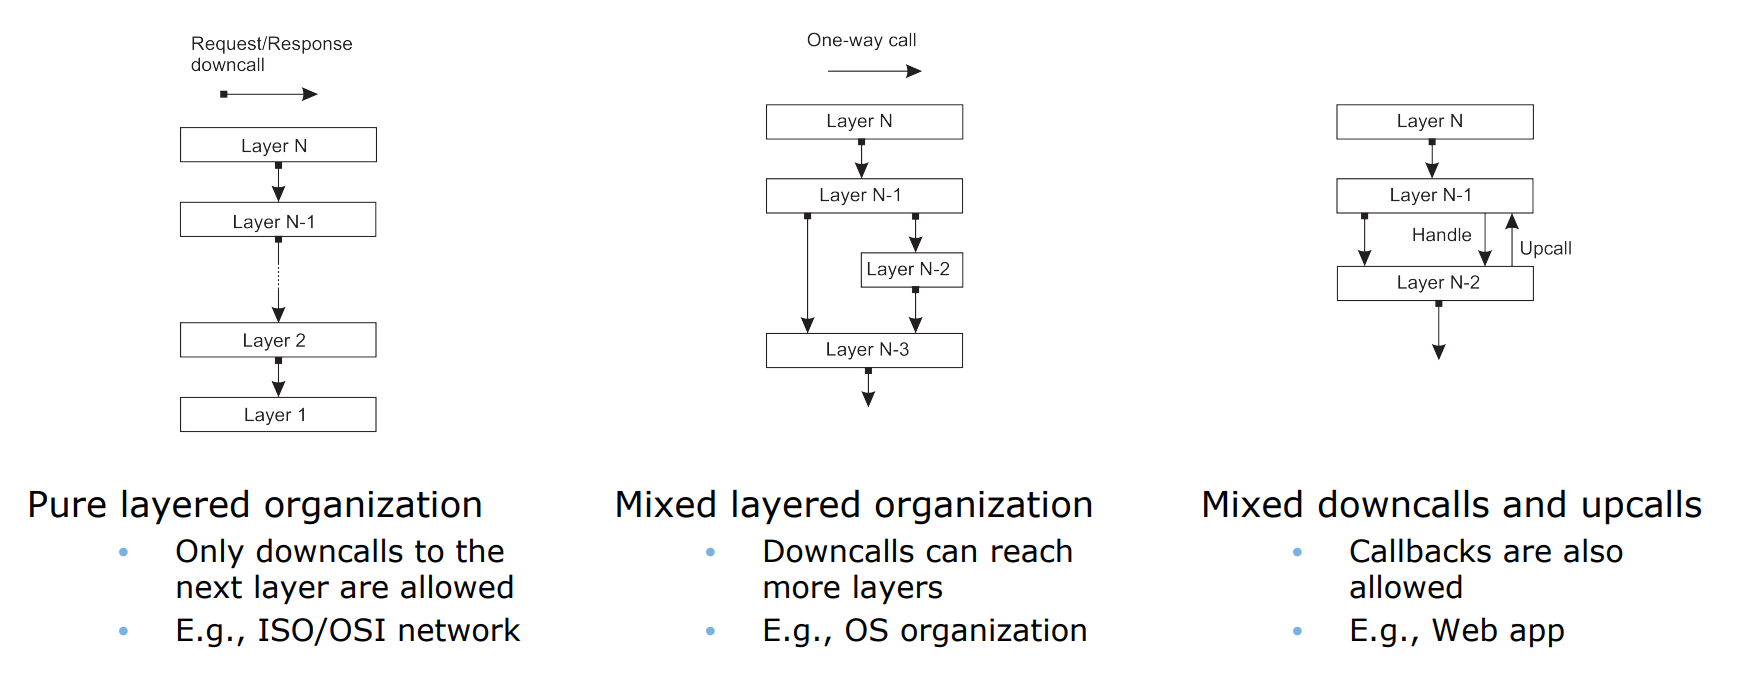
\includegraphics[scale=0.32]{layered.png}

    \begin{itemize}
        \item Il primo caso è molto semplice. Abbiamo a disposizione N livelli di layer, ognuno che comunica
        solo ed esclusivamente con il livello sottostante.
        \item Il secondo caso invece potrebbe risultare un po più complicato. Per spiegarlo usiamo un semplice esempio:
        supponiamo che il nostro programma effettui una operazione di divisione per 0 (zero).
        Ovviamente sappiamo che ciò non è possibile, quindi passerà il compito di risolvere questa eccezione
        all'exception handler e successivamente tornerà a fare quello che doveva fare.
        Invece se effettuiamo una normale operazione che non genera eccezzioni ovviamente non dovrà fare la parte dell'exception handler.
        \item Per il terzo caso basti immaginare a come funziona AJAX o più in generale il funzionamento di una web app.
        Quindi chiamate al server con eventuale risposta e aggiornamento della UI.
    \end{itemize}

    \subsection{Diversi tipi di Sistemi Distribuiti}
    E' importante differenziare i 3 tipi principali di SD.
    \begin{itemize}
        \item DOS (Distributed Operating System)
        \item NOS (Network Operating System)
        \item Middleware
    \end{itemize}  
    
    \subsection*{Distributed Operating System}
    L'utente non è a conoscenza della molteplicità delle macchine che compongono il sistema.
    \\I dati possono essere spostanti in modo intero o parziale, così come le operazioni di computazione.
    \\Un processo può essere migrato interamente o in modo parziale su diversi siti, facendo così avremo un effetto
    di \textbf{Load balancing}, che ci permette di distribuire il carico di lavoro su più macchine, 
    e di \textbf{Compuatation speedup} (i sottoprocessi possono essere eseguiti concorrentemente su più siti).
    Però il processo potrebbe aver bisogno di un determinato hardware (\textbf{Hardware preference}) oppure
    di un determinato software (\textbf{Software preference}). Avendo la possibilità di migrare il processo
    questo può essere possibile. 
    Infine il processo può essere eseguito in modo remoto, invece che trasferire i dati in locale.
    \newpage
    \subsection*{Network Operating System}
    L'utente è a conoscenza della molteplicità delle macchine che compongono il sistema.
    \\NOS permette operazioni esplicite di comunicazione: \textbf{Socket}.
    (Comunicazione diretta tra processi.)
    \\L'accesso alle risorse sulle varie macchine è effettuata in modo esplicito tramite:
    \begin{itemize}
        \item Remote logging (telnet, ssh)
        \item Remote desktop
        \item FTP
    \end{itemize}
    \subsection*{Middleware}
    Il compito del middleware è quello di implementare i servizi per renderli trasparenti all'applicazione.
    \begin{itemize}
        \item Definisce e offre un modello di comunicazione che nasconde i dettagli dei messaggi passati.
        \item Definisce e offre un servizio automatico per il salvataggio dei dati (su file system o DB).
        \item Definisce e offre un modello persistente per garantire consistenza su operazioni di lettura e scrittura (di solito su DB).
        \item Definisce e offre modelli di protezione nell'accesso ai dati e servizi.
    \end{itemize}
    \newpage
    \section{Il Modello Client-Server}

    \begin{figure}[htbp]
        \centering
        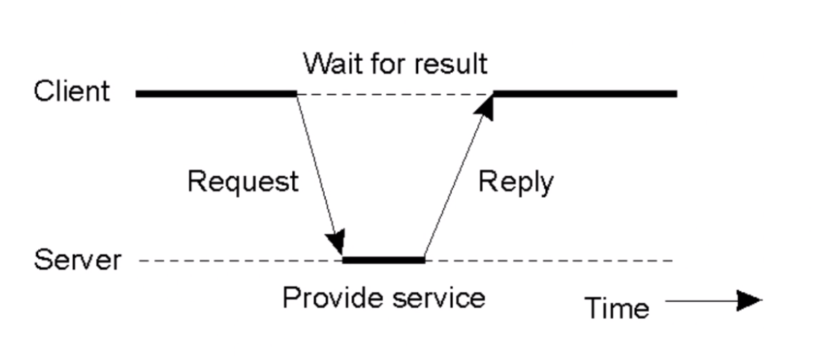
\includegraphics[scale=0.5]{clientserver.png}  
    \end{figure}
    Di base questa architettura prevede che un \textbf{client} acceda ad un \textbf{server} con
    una richiesta e che il server risponda con un risultato.
    \\Come possiamo notare dall'immagine, chiaramenta la richiesta con annessa risposta
    non è immediata, dovrà trascorrere un determinato quanto di tempo affinchè il server
    riesca a soddisfare la richiesta del client.
    \\\\
    Ci possono essere diversi tipi di modelli.

    \begin{itemize}
        \item \textbf{Accesso a Server multipli}.
        \\Il client accede ad un server che a sua volta può accedere ad un altro
        server. 
        \begin{figure}[htbp]
            \centering
            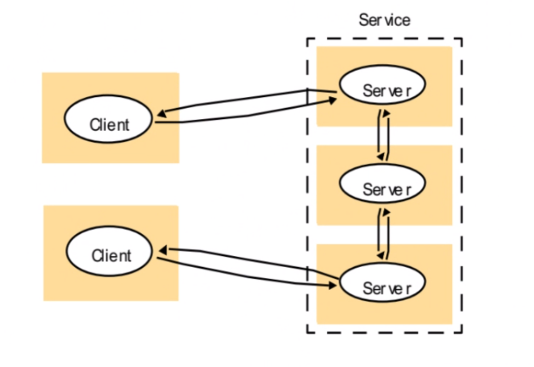
\includegraphics[scale=0.5]{servermultipli.png}  
        \end{figure}
        \newpage
        \item \textbf{Accesso via Proxy}
        \\Il \textit{Proxy} è un tipo di server che funge da intermediario per le richieste
        da parte di client alla ricerca di risorse su altri server.
        \\Il Server Proxy è molto utile per fornire l'anonimato durante la navigazione.
        \begin{figure}[htbp]
            \centering
            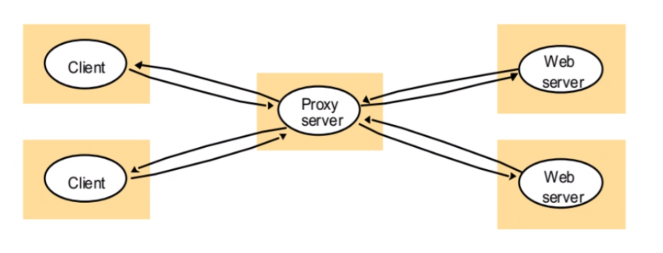
\includegraphics[scale=0.5]{proxy.png}  
        \end{figure}
    \end{itemize}
    
    \subsection{Problemi Fondamentali}
    In generale, ogni Sistema Distribuito deve aver a che fare con 4 problemi fondamentali:
    \begin{itemize}
        \item \textbf{Namig} (Identificare la controparte)
        \\Chi è la mia controparte? Dobbiamo assegnare dei nomi

        \item \textbf{Access point} (Accedere alla controparte)
        \\Come posso accedere ad una risorsa remota o un processo?

        \item \textbf{Protocol} (Comunicazione)
        \\Come posso scambiare messaggi? Bisogna mettersi d'accordo sul formato

        \item \textbf{Still an open issue} (Comunicazione)
        \\Come posso capire il contenuto di un messaggio?
    \end{itemize}

    \subsection{Trasparenza}
    Il concetto fondamentale alla base di un buon Sistema Distribuito è, appunto,
    la trasparenza. Per cui, per esempio, il come un particolare dato venga rappresentato
    e la metodologia di accesso a quel dato sono \textit{trasparenti} all'utente, non li vede.
    Così come anche la \textit{location}. Non sappiamo dove quel dato risiede fisicamente.
    \\\\Però, avere un \textbf{grado} di trasparenza troppo elevato potrebbe risultare eccessivo.
    Per esempio:
    \begin{itemize}
        \item Alcune \textit{latenze di comunicazione} non possono essere nascoste.
        \item Nascondere i fallimenti del sistema e dei nodi è talvolta \textbf{impossibile}.
        \item Esporre le distribuzioni potrebbe essere alcune volte una buona pratica.
        \\Se un server non dovesse rispondere ad una chiamata per troppo tempo, bisogna riportare il fallimento
        per dare un feedback all'utente di cosa sta accadendo e di agire di conseguenza.
        \item Inoltre, la trasparenza completa ha un costo elevato 
        (e.g.\ Mantenere le repliche di tutti i dati esattamente "up-to-date" con il master)
    \end{itemize}

    \subsubsection{Information Hiding}
    L'Information Hiding è il principio che sta alla base dell'\textit{Ingegneria del Software}.
    \\E' importante fare una distinzione tra:
    \begin{itemize}
        \item \textbf{cosa} un servizio o un sistema mette a disposizione
        \\definisce l'\textit{Application Programming Interface} (API) dei componenti o del sistema.
        \item \textbf{come} un servizio è stato implementato e distribuito
        \\definisce come il tool adatto per quel specifico problema.
    \end{itemize}
    
    Queste interfacce però devono essere sviluppate seguendo certi criteri, 
    quindi devono mantenere una struttura che segua i principi prestabiliti,
    deve essere completa (mettere a disposizione tutto quello che serve) e neutrale.

    \subsection{Il concetto di Protocollo}
    Per poter capire le richieste e formulare le risposte i due processi devono concordare
    un \textbf{protocollo}.
    \\I protocolli definiscono il \textbf{formato}, l'\textbf{ordine} di invio e di ricezione dei messaggi,
    il \textbf{tipo dei dati} e le \textbf{azioni} da eseguire quando si riceve un messaggio.
    \\Alcuni esempi di protocolli sono:
    \begin{itemize}
        \item HTTP - HyperText Transfer Protocol
        \item FTP - File Transfer Protocol
        \item SMTP - Simple Mail Transfer Protocol
    \end{itemize}
    
    \section{Le Socket}
    I processi sono i programmi in esecuzione, che sono aree di memoria gestite dal Sistema Operativo.
    Ogni processo comunica attraverso dei \textbf{canali},
    che controllano i \textit{flussi di dati in \textbf{entrata} e \textbf{uscita}}.
    \\Dall'esterno, ogni canale è identificato da un numero intero detto \textbf{porta}.
    \\\\
    Le \textbf{socket} sono dei particolari canali per la comunicazione tra \textit{processi} che non condividono memoria.
    \\Per potersi connettere o inviare dati ad un processo A, un processo B deve conoscere la macchina (\textit{host})
    che esegue A e la porta a cui A è connesso. (\textit{Well known port (?)})
    \\\\
    
    \subsection{Servizi di trasporto di dati}

    \subsubsection*{TCP}
    Il servizio \textit{TCP} è un protocollo \textbf{orientato alla connessione}, ovvero 
    che il \textit{client} invia al \textit{server} una richiesta di connessione, e il server
    risponde di conseguenza.
    \\TCP è famoso per il suo \textbf{trasporto affidabile}, tra la comunicazione tra processi.
    \\Possiede anche un \textbf{controllo di flusso} (il mittente rallenta per non sommergere il ricevente)
    e un \textbf{controllo della congestione} (il mittente rallenta quando la rete è sovraccaricata).
     
    \subsubsection*{UDP}
    UDP è un protocollo che \textbf{non} garantisce la ricezione del messaggio, e 
    in generale \textbf{non} possiede tutte le funzionalità di sicurezza del TCP.
    \\Quindi, \textit{perchè esiste UDP?}
    \\UDP può essere molto utile per le applicazioni che tollerano perdite parziali
    (ad esempio un servizio di video streaming, anche se perdiamo qualche frame non ci accorgiamo nemmeno)
    a vantaggio delle prestazioni.
    \\\\
    Le socket non sono altro che delle API per accedere ai servizi di trasporto TCP e UDP.
    \\\\
    \subsection{Comunicazione via socket}
    La comunicazione TCP/IP avviene attraverso \textbf{flussi di byte} dopo una
    \textbf{connessione esplicita}, tramite normali \textit{System Call} di read/write.

    \begin{figure}[htbp]
        \centering
        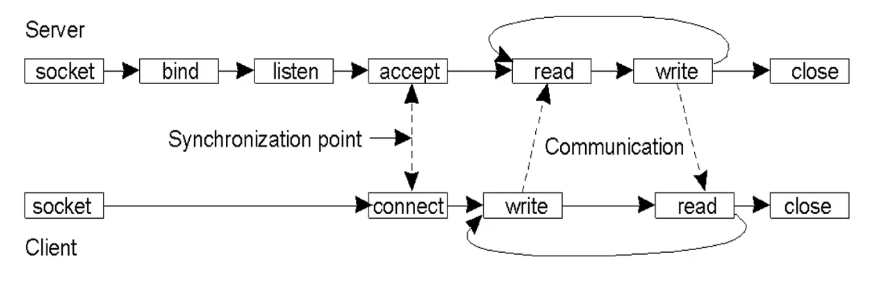
\includegraphics[scale=0.7]{socketsteps.png}
    \end{figure}

    \begin{itemize}
        \item \textbf{Socket}: viene creata un nuovo canale socket.
        \item \textbf{Bind}: viene associato un \textit{local address (porta)} alla socket per l'identificazione del processo
        \item \textbf{Listen}: si mette in ascolto di nuove connessioni
        \item \textbf{Connect}: il client invia una richiesta di connessione al server
        \item \textbf{Accept}: accetta la connessione del client.
        \\Crea una nuova porta per gestire la \textbf{comunicazione} (dedicata). 
        \item \textbf{Write}: invia dei dati attraverso il canale
        \item \textbf{Read}: riceve dei dati attraverso il canale
        \item \textbf{Close}: chiude la connessione
    \end{itemize}
    La \textbf{comunicazione} è un ciclo continuo di \textit{read} e \textit{write}
    tra il client e il server fino a che non viene chiusa la connessione.
    \\Le socket trasportano degli \textit{stream}, quindi non esiste il concetto di messaggio,
    è appunto un flusso continuo di dati.
    \\Però la lettura e la scrittura avvengono per un numero arbitrario di byte.
    \\\\
    \textbf{Connect} e \textbf{Accept} "bloccano" il sistema (rispettivamente il client e il server)
     fino a che non viene stabilita una connessione (vengono messi in attesa).
    \\\\
    \newpage
    \textit{Perchè non viene creata solo una porta per la comunicazione ma ne vengono create molteplici?}
    \\\\Per gestire e identificare le varie connessioni che sono state create tra i client che si sono collegati al server.

    \begin{figure}[htbp]
        \centering
        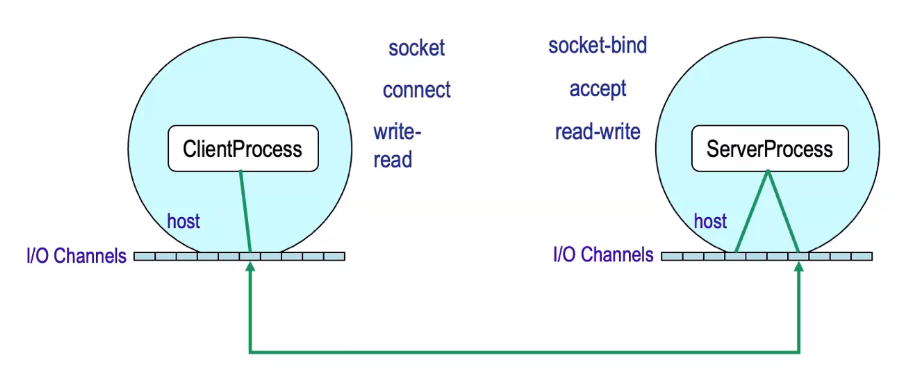
\includegraphics[scale=0.6]{socketsteps2.png}
    \end{figure}

    \subsection{Progettare una Applicazione con le Socket}
    \begin{itemize}
        \item \textbf{Client}: L'architettura è più semplice di quella di un server:
        \\di solito è una applicazione che usa una socket anzichè un altro canale I/O
        \item \textbf{Server}: L'architettura prevede che:
        \begin{itemize}
            \item venga creata una socket con una porta nota per accettare le richieste di connessione
            \item entri in un ciclo infinito in cui alternare:
            \begin{itemize}
                \item attesa/accettazione di una richiesta di connessione da un client
                \item ciclo lettura-esecuzione
                \item chiusura connessione
            \end{itemize}        
        \end{itemize}
    \end{itemize}

    \newpage

    \section{Architettura dei Server}
    I server possono essere:
    \begin{itemize}
        \item \textbf{Iterativi}: soddisfano una richiesta alla volta
        \item \textbf{Concorrenti a processo singolo}: simulano la presenza di un server dedicato
        \item \textbf{Concorrenti multi-processo}: creano server dedicati
        \item \textbf{Concorrenti multi-thread}: creano thread dedicati
    \end{itemize}

    \subsection{Server Iterativi}
    Al momento di una richiesta di connessione, il server crea una socket 
    temporanea per stabilire una connessione diretta con il client.
    \\Eventuali ultieriori richieste, verranno accodate alla porta nota per essere soddisfatte in seguito.
    \\\\
    Questa architettura ha il \textbf{vantaggio} che è molto semplice da progettare, \textbf{però} viene servito un client alla volta,
    mettendo appunto in attesa gli altri. 

    \subsection{Server Concorrenti}

    Un server concorrente può gestire più connessioni client.

    \begin{itemize}
        \item \textbf{Monoprocesso}:
        Esistono delle funzioni (\textit{select in C}) che vanno a selezionare i canali pronti all'uso.
        \begin{figure}[htbp]
            \centering
            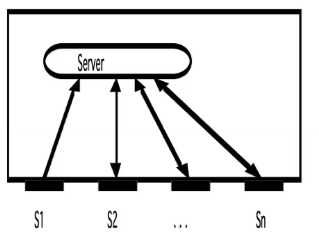
\includegraphics[scale=0.7]{monoprocesso.png}
            
        \end{figure}
        \\S1 è la socket per accettare le richieste di connessione, le altre sono le connessioni individuali.
        \\Nei server monoprocesso, gli utenti condividono lo stesso spazio di lavoro, quindi adatto
        per le applicazioni cooperative che prevedono la modifica dello stato
        
        \item \textbf{Multi-thread}:
        \\Ho un processo singolo, e all'interno dei piccoli sotto processi (Thread) che simulano un processo a se

        \begin{figure}[htbp]
            \centering
            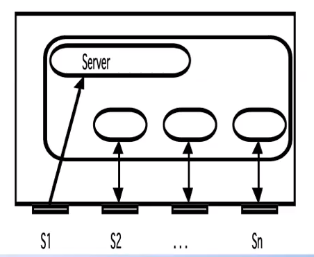
\includegraphics[scale=0.5]{multithread.png}
        \end{figure}

        \item \textbf{Multi-processo}:
        Ho degli effettivi processi clone, quindi veri e propri server "fisici", non simulati.

        \begin{figure}[htbp]
            \centering
            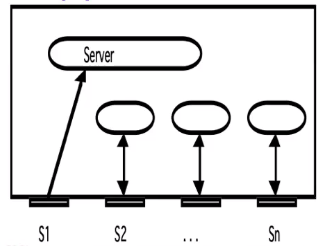
\includegraphics[scale=0.5]{multiprocesso.png}
            
            
        \end{figure}
        Nei server multiprocesso, ogni utente ha uno spazio di lavoro autonomo, quindi adatto
        per le applicazioni che non modificano lo stato del server, oppure per quelle applicazioni
        che prevedono una modifica solamente al proprio spazio di lavoro dedicato.
    \end{itemize}
    \newpage
    Per quanto riguarda la funzione di \textit{select}, essa permette di gestire in modo non bloccante
    i diversi canali di I/O.
    \\(Una istruzione \textit{bloccante} è quando il sistema attende la conclusione dell'operazione 
    richiesta prima di restituire il controllo al chiamante)

    \begin{figure}[htbp]
        \centering
        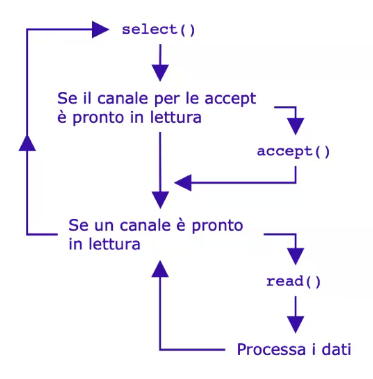
\includegraphics[scale=0.66]{select.png}
    \end{figure}

    \subsection*{Struttura di un Server Concorrente}
    \begin{figure}[htbp]
        \centering
        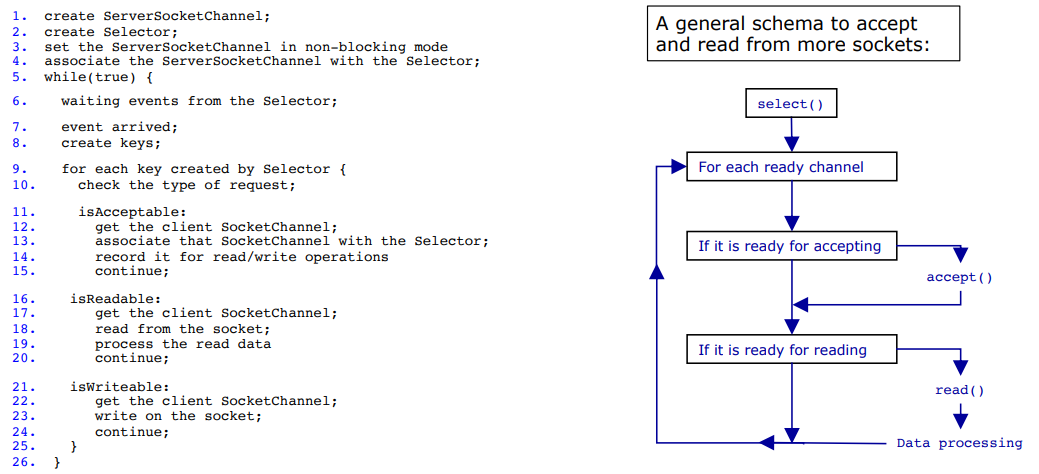
\includegraphics[scale=0.55]{serverconcorrente.png}
        \caption{Un esempio di codice pratico lo puoi trovare al seguente link: \url{https://github.com/LeoRc01/Concurrent-Socket}}
    \end{figure}

    \section{Architettura del Web}
    Il web supporta l'interazione tra Client e Server attraverso il protocollo HTTP.
    \begin{itemize}
        \item Il client è formato da \textit{browser} oppure anche chiamato \textbf{User-agent}
        \item Il server è formato ad un \textit{web server} o \textbf{HTTP Server}
    \end{itemize}
    
    \subsection{Browser}
    Il browser è una applicazione che consente al client di navigare sul web.
    \\La sua funzione primaria è quella di \textbf{interpretare} il codice con cui sono espresse 
    le informazioni (pagine web) e \textbf{visualizzarle} sullo schermo.

    \subsection{Web page}
    Una pagina web è costituita da diversi risorse. Una risorsa è un file residente in un computer
    identificato da un URL, ovvero un indirizzo univoco che punta alla risorsa. 
    \\La maggior parte delle pagine web sono costituite da un file HTML.

    \subsection{Web server}
    Un web server è una applicazione che si occupa di gestire le risorse su un computer 
    e di renderle disponibili al client
    \newpage
    \subsection{URL (Uniform Resource Locator)}
    \textbf{Identifica} un oggetto nella rete e specifica come interpretare i dati ricevuti
    attraverso il protocollo.
    \\Un URL ha cinque componenti principali:
    \begin{itemize}
        \item Nome del protocollo
        \item Indirizzo dell'host
        \item Porta del processo
        \item Percorso dell'host
        \item Identificatore della risorsa
    \end{itemize}

    \begin{figure}[htbp]
        \centering
        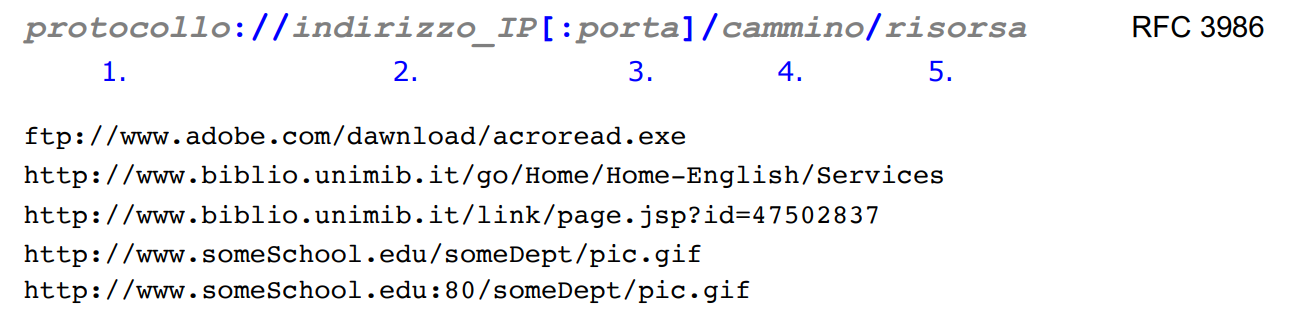
\includegraphics[scale=0.5]{url.png}
    \end{figure}

    \subsection{Linguaggi del web}
    I \textbf{dati} testuali sono espressi in linguaggi standard:
    \begin{itemize}
        \item HTML - per definire la struttura dei contenuti della pagina web.
        \\\\Un file HTML può contenere (nella maggior parte dei casi) dei contenuti scritti
        in CSS (gestisce la parte grafica e di "rendering")
        \item XML | JSON - focalizzato sui dati e la loro struttura
    \end{itemize}
    I dati possono anche essere non testuali (file di immagini, file di audio, file di video, ecc.)
    Essi vengono gestiti attraverso dei sistemi di \textit{Encoding}.
    \\\\
    Esistono anche dei linguaggi di scripting (JavaScript, VBSCript, Java, ecc.) che permettono 
    di arricchire la pagina web di funzionalità più complesse che magari non possono essere implementate
    esclusivamente attraverso HTML e CSS.

    \section{Message Oriented Comunication}
    \subsection{Il protocollo HTTP}
    HTTP (o anche HTTPS) è il protocollo standard per la comunicazione, e lo scambio di risorse,
    tra client e server. HTTP usa TPC per la comunicazione.
    \begin{itemize}
        \item Il client inizia una connessione TCP (crea una socket) verso il server sulla porta 80 (443 nel caso di HTTPS)
        \item Il server accetta la connessione TCP dal client
        \item Vengono scambiati i messaggi tra il browser e il Web-server
    \end{itemize}

    \begin{figure}[htbp]
        \centering
        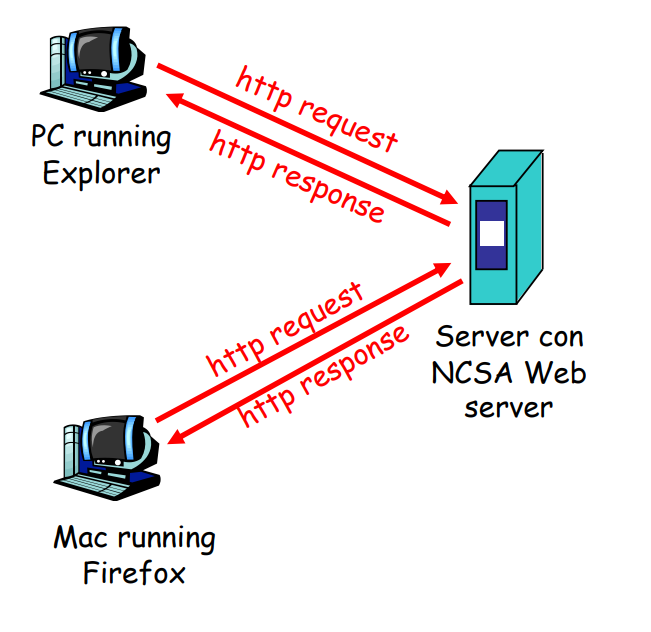
\includegraphics[scale=0.5]{http.png}
    \end{figure}
    
    HTTP è un protocollo \textbf{stateless}, ovvero che non mantiene in memoria informazioni sul client.
    
    \newpage
    \subsection{Formato dei messaggi HTTP}

    Formato \textbf{generale} di un messaggio HTTP:
    \begin{figure}[htbp]
        \centering
        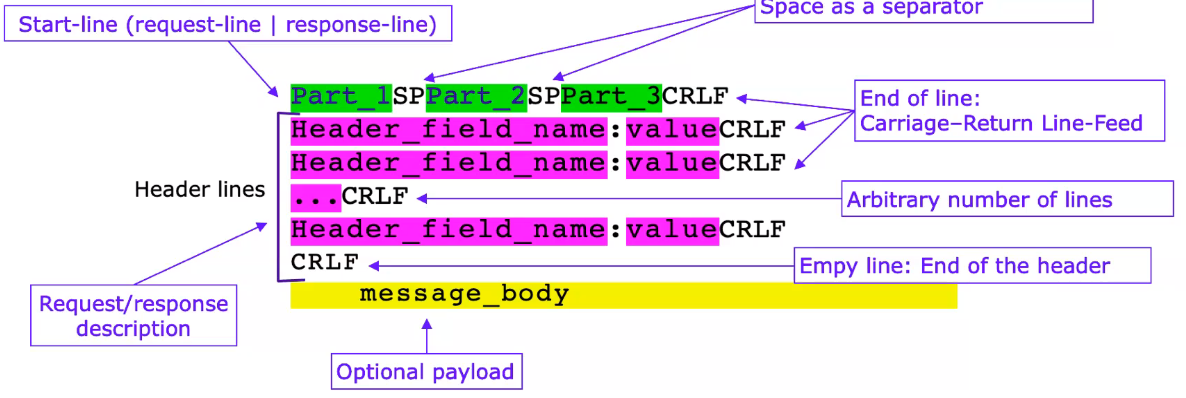
\includegraphics[scale=0.5]{httpgeneral.png}
    \end{figure}
    \\La prima parte in verde è \textbf{obbligatoria}.
    \\La parte gialla è il \textbf{payload} (il contenuto del messaggio).

    Formato di una richiesta HTTP:
    \begin{figure}[htbp]
        \centering
        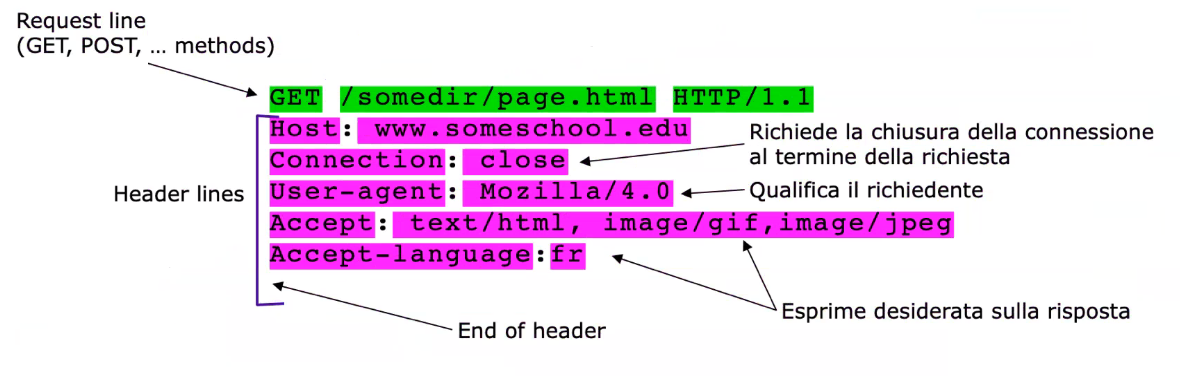
\includegraphics[scale=0.5]{httprequest.png}
    \end{figure}
    
    \begin{itemize}
        \item \textbf{GET} - metodo della richiesta
        \item \textbf{/somedir/page.html} - percorso della risorsa
        \item \textbf{HTTP/1.1} - versione del protocollo
        \item \textbf{Host: www.someschool.edu} - URL del server
        \item \textbf{Connection: close} - cosa fare al termine del messaggio (in questo caso chiudere la connessione)
        \item \textbf{User-Agent: Mozilla/4.0} - il browser utilizzato dal client
        \item \textbf{Accept: text/html, image/gif, image/jpeg} - che tipi di file sono accettati
        \item \textbf{Accept-Language: fr} - linguaggio della risorsa richiesta. (Se hai la risorsa francese, mandamela in francese).
    \end{itemize}

    \subsection*{Metodi di richiesta}
    \begin{itemize}
        \item \textbf{GET}
            \begin{itemize}
                \item Restituisce la risorsa richiesta
                \item Include eventuali parametri in coda alla URL della risorsa
                \item L'esecuzione non ha effetti sul server
                \item Esiste anche il \textbf{GET Condizionale}, ovvero non inviare oggetti che il client ha già in cache
            \end{itemize}
            \item \textbf{POST}
            \begin{itemize}
                \item Comunica dei dati da elaborare lato server
                \item L'input segue come documento autonomo
                \item I parametri passati non vengono mostrati esplicitamente
            \end{itemize}
            \item \textbf{HEAD}
            \begin{itemize}
                \item Simile a GET, ma viene restituito solo il header della pagina web
                \item Usata per il \textbf{debugging}
            \end{itemize}
    \end{itemize}

    \begin{figure}[htbp]
        \centering
        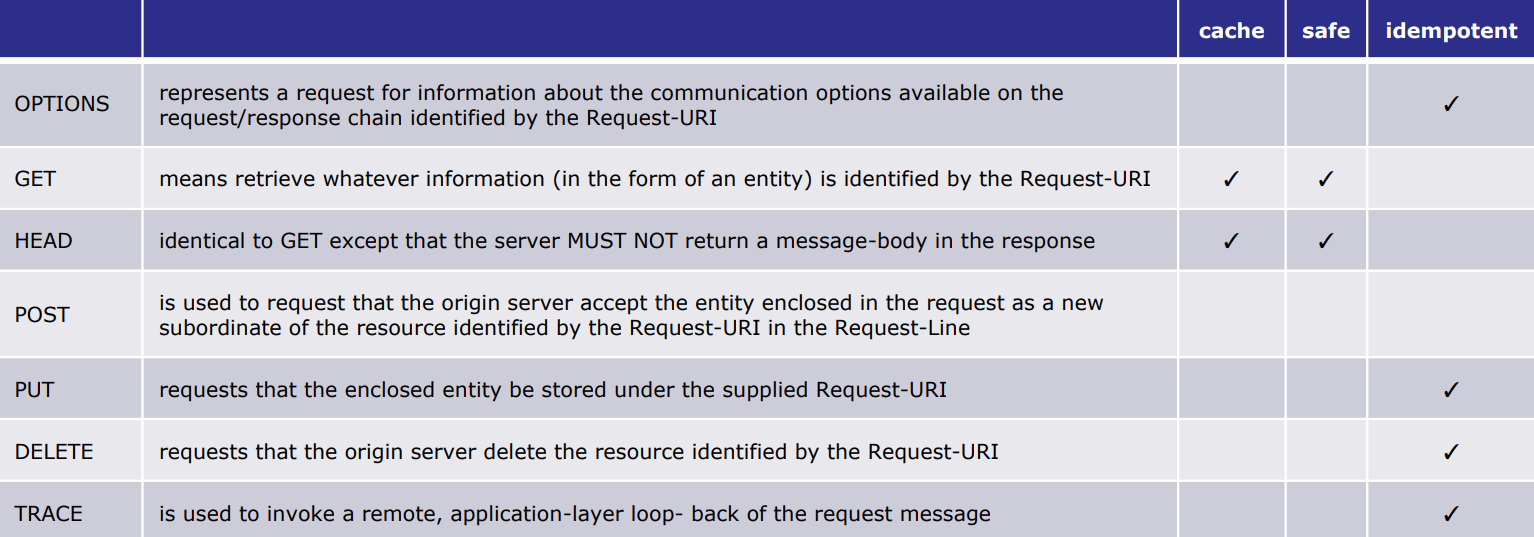
\includegraphics[scale=0.4]{metodi.png}
    \end{figure}

    \newpage
    Formato di una response HTTP:
    \begin{figure}[htbp]
        \centering
        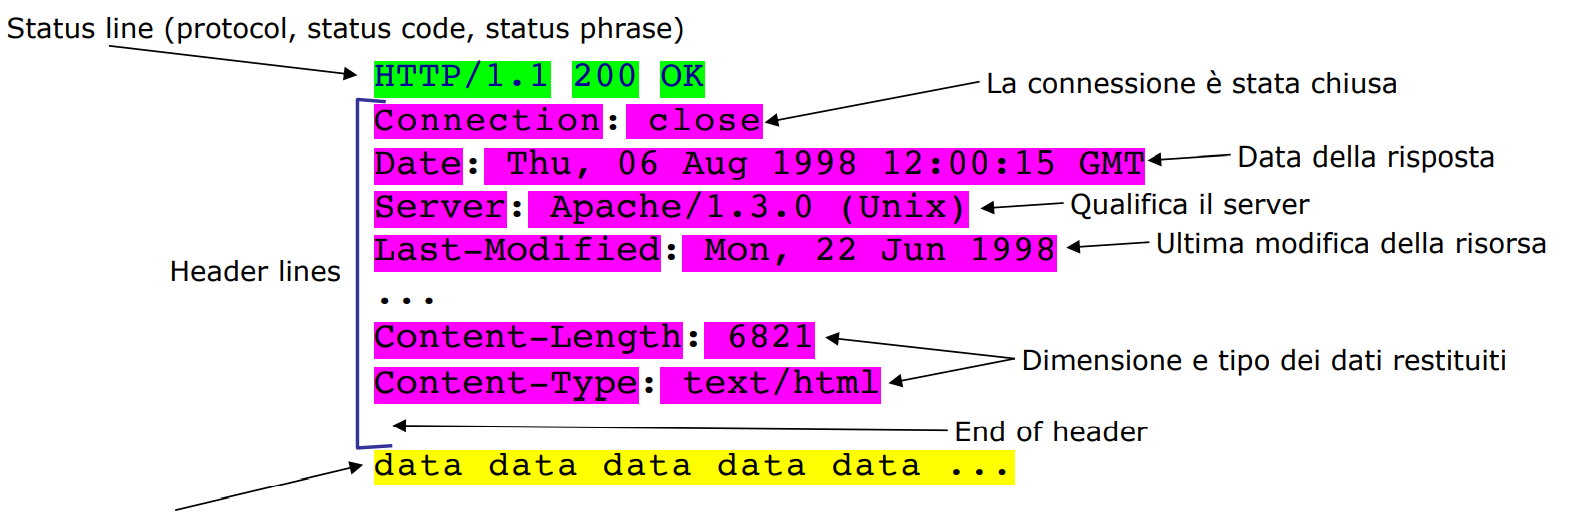
\includegraphics[scale=0.4]{httpresponse.png}
    \end{figure}

    \textbf{Perchè sono state inserite informazioni sulla dimensione e sul tipo dei dati restituiti?}

    \begin{itemize}
        \item \textbf{Lenght} - mi serve per vedere fino a quando devo leggere
        \item \textbf{Type} - per far capire al client come deve interpretare la risposta
    \end{itemize}

    \subsection{Codici di risposta}
    \begin{figure}[htbp]
        \centering
        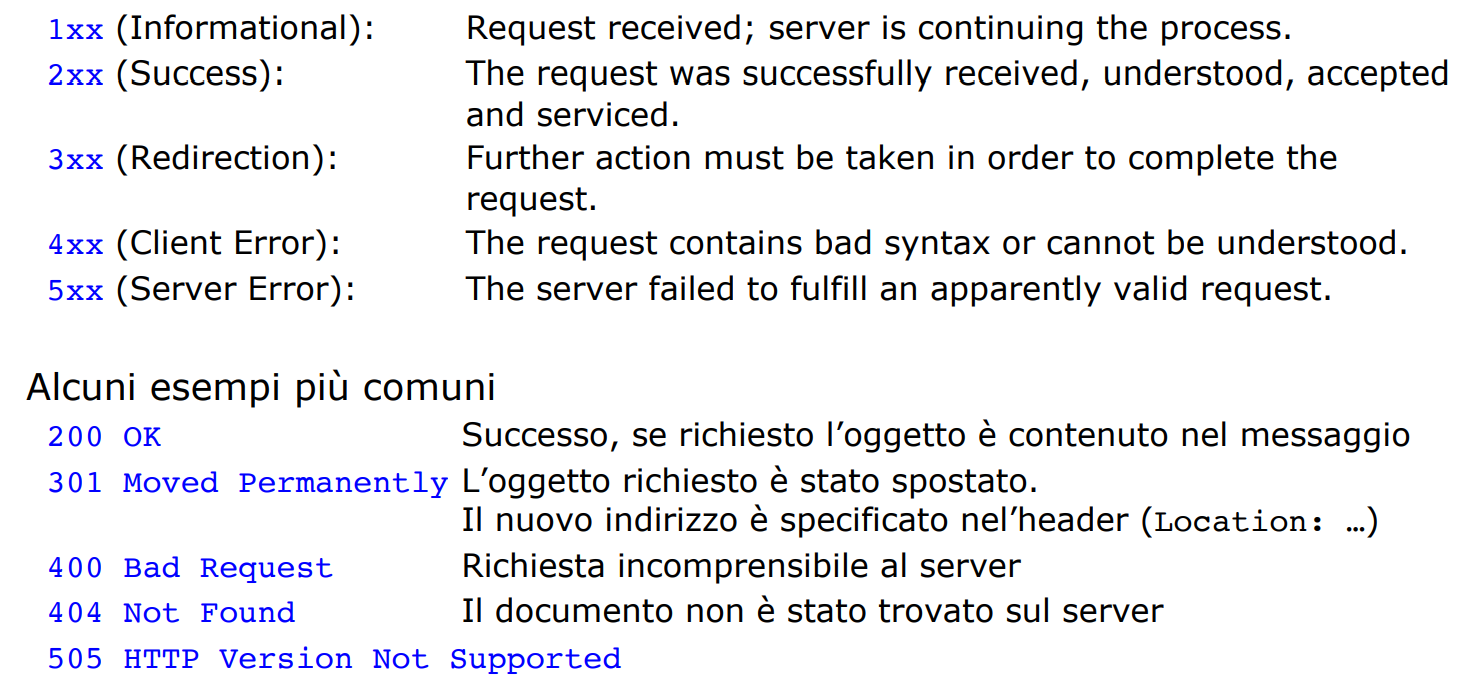
\includegraphics[scale=0.4]{codici.png}
    \end{figure}    








    \newpage
    \section{HTML+(DOM+)CSS}
    \subsection{Linguaggi di Markup}
    Un linguaggio di Markup è utilizzato per \textit{annotare un documento} in modo 
    tale che l'annotazione sia \textit{sintatticamente distinguibile} dal testo.
    \\Le annotazioni possono avere diverse finalità:
    \begin{itemize}
        \item Presentazione (definiscono come visualizzare il testo)
        \item Precedurali (definiscono istruzioni per programmi che elaborino il testo al quale sono associate)
        \item Descrittive (metadati, possono servire per il browser per identificare alcune informazioni, etichettano semplicemente parti del testo, )
    \end{itemize}


    \subsection{HTML}
    HyperText Markup Language è un linguaggio di markup per \textbf{dare struttura ai contenuti} del web.
    La struttura data al contenuto viene esplicitata tramite i \textbf{tag}. Essi \textit{delimitano}
    dei pezzi di documento e possono essere composti da altri tag. Ogni tag ha un suo particolare effetto.
    \\In assenza di CSS, il browser si "arrangia" nel dare una rappresentazione grafica standard del documento.

    \subsection{CSS}
    Cascading Style Sheets è un linguaggio di markup per \textbf{definire uno stile} ai contenuti del web.
    \begin{figure}[htbp]
        \centering
        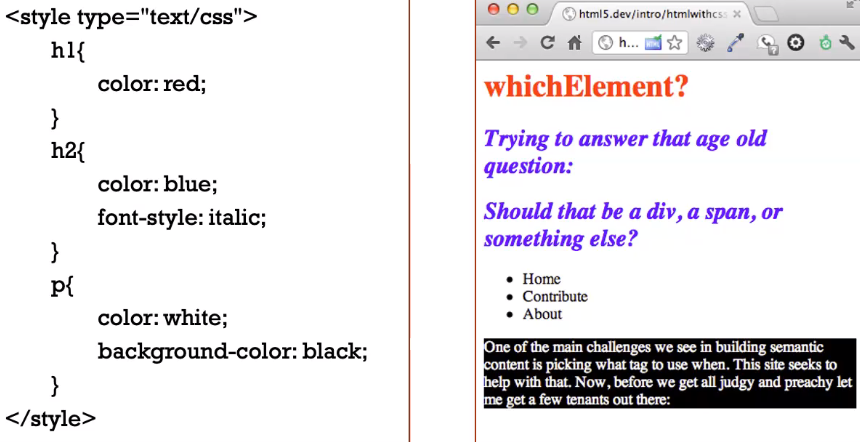
\includegraphics[scale=0.5]{css.png}
    \end{figure}

    \subsubsection{Selectors}
    Possiamo specificare un selettore più preciso rispetto al nome del tag.
    \begin{figure}[htbp]
        \centering
        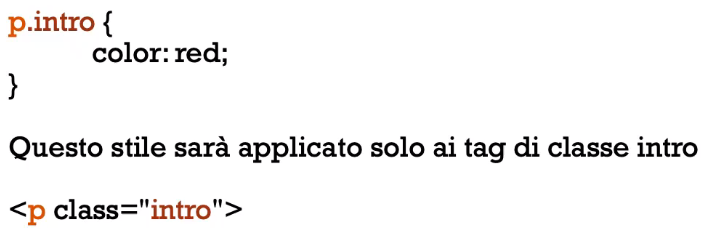
\includegraphics[scale=0.5]{selector.png}
        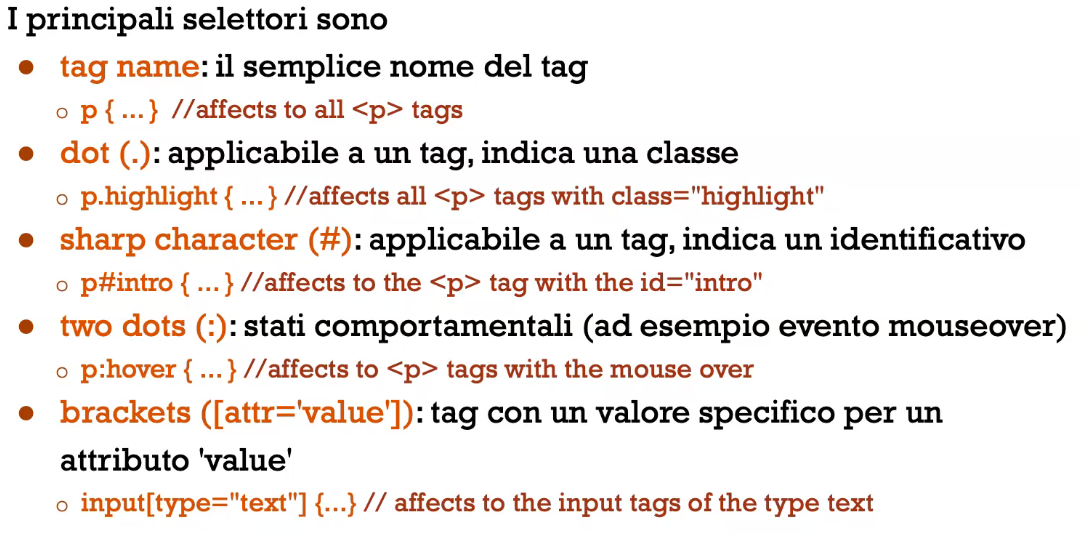
\includegraphics[scale=0.5]{selectors.png}
    \end{figure}

    \subsubsection{Media Query}
    Le media query possono essere viste come particolari selettori capaci di 
    \textbf{valutare le capacità del device} di accesso alla pagina.
    \\Servono per controllare ad esempio:
    \begin{itemize}
        \item Larghezza e Altezza del device
        \item Orientamento dello schermo
        \item Risoluzione
    \end{itemize}
    Oggi come oggi, gli stili dei siti web sono \textit{responsive}, ovvero che lo stile
    di rappresentazione della pagina varia in base alla larghezza dello schermo. 
    (Quindi in base al device di accesso alla pagina).

    \subsubsection{Perchè cascading?}
    Esistono potenzialmente diversi stylesheets:
    \begin{itemize}
        \item L'autore della pagina in genere ne specifica uno o pià di uno
        \item Il browser ne ha uno, o un vero e proprio CSS o simulato nel loro codice
        \item Il lettore, l'utente del browser ne può definire uno proprio per customizzare la propria esperienza
    \end{itemize}
    Sono quindi inevitabili dei \textbf{conflitti} ed è necessario definire un algoritmo per decidere quale stile vada applicato ad un elemento.

    \subsection{DOM}
    Document Object Model è una \textbf{interfaccia neutrale} rispetto al linguaggio di programmazione e alla piattaforma utilizzata
    per consentire ai programmi l'accesso e la modifica dinamica di \textbf{contenuto, struttura e stile} di un documento del web.
    \\
    Ogni nodo può essere caratterizzato da attributi che ne facilitano l'identificazione, la ricerca,
    la selezione:
    \begin{itemize}
        \item \textbf{Identificatore Univoco}
        \item \textbf{Classe} che indica l'appartenenza ad un insieme che ci è utile definire
    \end{itemize}



    

\end{document}